\section{Up-Sets and Down-Sets}
\label{section_1.6}

\begin{definition}
  Let $P$ be a poset , and $Q \subseteq P$ a poset under the induced
  order. We call $Q$ a \textbf{down-set} if for every $x \in Q$, if $y
  \in P$ such that $y \leq x$, then $y \in Q$. Similarly, we call $Q$
  an \textbf{up-set} if for every $x \in Q$, if $y \in P$ such that $x
  \leq y$, then $y \in Q$. We define $\down{Q}=\{ y \in P : y \leq x
  \text{ for some } x \in Q\}$ and $\up{Q}=\{ y \in P : x \leq y
\text{ for some } x \in Q\}$. Similarly, $\down{x}=\{y \in P : y \leq
x\}$ and $\up{x}=\{y \in P: x \leq y\}$. We denote by $\Oc(P)$ the set
of all down-sets in $P$.
\end{definition}

\begin{lemma}\label{lemma_1.6.1}
  Let $P$ be a poset. Then  $\Oc(P)$ is a poset under inclusion.
\end{lemma}
\begin{proof}
  It suffices o show that down-sets are closed under inclusion; that
  is, if $Q$ is a down-set, and $R \subseteq Q$, then $R$ is also a
  down-set.

  Indeed, let $Q \in \Oc(P)$ and $R \subseteq Q$. Let $x \in M$, and
  $y \in P$ such that $y \leq x$. Since $x \in M$, $x \in Q$, so by
  definition of $Q$ as a down-set, $y \in Q$. Then we have that $y
  \leq x$, and $x \in M \subseteq Q$. By definition of a down-set
  again, we must have $y \in M$.

  For ordering, observe that $\Oc(P)$ inherits the induced order of
  $2^P$.
\end{proof}
\begin{corollary}
  If $Q \subseteq P$ is any set, then $\down{Q}$ is the smallest
  down-set containing $Q$. Moreover,  $Q \in \Oc(P)$ if, and only if
  $Q=\down{Q}$. Moreover, $\down{\{x\}}=\down{x}$.
\end{corollary}
\begin{proof}
  Let $y \in \down{Q}$, then there is some $x \in Q$ for which $y \leq
  x$. Now, let $z \in P$ such that $z \leq y$ so that $z \leq y \leq
  x$. By definition, this puts $z \in \down{Q}$ and makes $\down{Q}
  \in \Oc(P)$.

  Observe now, that if $x \in Q$, then $x \in P$ and by reflexivity $x
  \leq x$ which puts $x \in \down{Q}$, and hence $Q \subseteq
  \down{Q}$. Suppose now, there is a down-set $R$ such that $Q
  \subseteq R \subseteq \down{Q}$. Choose $y \in \down{Q}$, then there
  exists an $x \in Q$ for which $y \leq x$ in $Q$. Since  $Q \subseteq
  R$, $y \leq x$ in $R$, which puts  $y \in R$ so that $R=\down{Q}$.

  Now, suppose that $Q$ is a down-set. We have that $Q \subseteq
  \down{Q}$, and since $\down{Q}$ is the smallest down-set containing
  $Q$, by the above argument,  $\down{Q}=Q$. Lastly, observe that
  $\down{\{x\}}=\{y \in P : y \leq x \text{ for some } x \in
  \{x\}\}=\{y \in P : y \leq x\}=\down{x}$.
\end{proof}
\begin{corollary}
  The set of up-sets of $P$ is the dual $\Oc(P)^\partial$ of the set
  of down-sets of $P$. Moreover for any $Q \subseteq P$, $\up{Q}$ is
  the largest up-set contained in $Q$, and  $Q \in \Oc(P)^\partial$
  if, and only if $Q=\up{Q}$, and $\up{\{x\}}=\up{x}$.
\end{corollary}
\begin{proof}
  This is the duality principle applied to the previous corollary.
\end{proof}

\begin{definition}
  Let $P$ be a poset and $Q \subseteq P$ have the induced order. We
  call $Q$ a \textbf{principle} down-set (up-set respectively) if
  there is some $x \in P$ for which $Q=\down{x}$ ($Q=\up{x}$,
  respectively).
\end{definition}

\begin{proposition}\label{proposition_1.6.2}
  Let $P$ be a poset, and $Q$ a non-empty down-set of  $P$. Then
  \begin{equation*}
    Q=\bigcup_{\a}{\down{x_\a}} \text{ where } x_\a \in \Max{Q}
  \end{equation*}
  Moreover, $\Max{Q}$ is an anti-chain.
\end{proposition}
\begin{proof}
  We prove first that $\Max{Q}$ is an anti-chain. Let $x,y \in
  \Max{Q}$ such that $x \leq y$. By maximality of $x$, we get  $x=y$
  (similarly, by maximality of $y$,  $y=x$). This makes $\Max{Q}$ an
  anti-chain.

  Now, let $y \in Q$, then by maximality, there exists at-least one
  $x_\a \in \Max{Q}$ (indexed by $\{\a\}$, not necessarily countable)
  for which $y \leq x_\a$. This puts $y \in \down{x_\a}$ so that $Q
  \subseteq \bigcup{\down{x_\a}}$. Moreover, notice that since $x_\a
  \in Q$ for all $\a$,  $\bigcup{\down{x_\a}} \subseteq Q$, and
  equality is established.
\end{proof}
\begin{corollary}
  If $P$ is finite, then
  \begin{equation*}
    Q=\bigcup_{k=1}^n{\down{x_k}} \text{ where } \Max{Q}=\{x_1, \dots,
    x_n\}
  \end{equation*}
  and we have
  \begin{equation*}
    |Q|=\sum_{k=1}^n{|\down{x_k}|}-\Big{|} \bigcap_{k=1}^n{\down{x_k}} \Big{|}
  \end{equation*}
\end{corollary}
\begin{proof}
  If $P$ is finite, then so is $Q$, and hence so is $\Max{Q}$. The
  size of $Q$ follows by counting the elements of $\bigcup{x_k}$,
  which may not be a disjoint union.
\end{proof}

\begin{example}\label{example_1.13}
  \begin{enumerate}
    \item[(1)] Consider the poset $P=\{a,b,c,d,e,f\}$ of example
      \ref{example_1.7}(2). The sets $\{c\},\{a,b,c,d,e\}$ and
      $\{a,b,d,f\}$ are all down-sets of $P$.
      $\down{\{b,d,e\}}=\{a,b,c,d,e\}$. The set $\{e,f,g\}$ is a
      up-set of $P$, but $\{a,b,d,f\}$ is not.

    \item[(2)] Let $P=\{a,b,c,d\}$. Then $P$ and  $\Oc(P)$ is
      represented by the diagrams below:
      \[\begin{tikzcd}[column sep=scriptsize]
        &&&&&& {\{a, b, c, d\}} \\
        P &&&&& {\{a,b,d\}} && {\{a,c,d\}} \\
        & b & c &&&& {\{a,d\}} && {\{c,d\}} \\
        & a & d &&& {\{a\}} && {\{d\}} \\
        &&&&&& \emptyset & {\Oc(P)}
        \arrow[no head, from=2-6, to=1-7]
        \arrow[no head, from=2-8, to=1-7]
        \arrow[no head, from=3-7, to=2-6]
        \arrow[no head, from=3-7, to=2-8]
        \arrow[no head, from=3-9, to=2-8]
        \arrow[no head, from=4-2, to=3-2]
        \arrow[no head, from=4-3, to=3-2]
        \arrow[no head, from=4-3, to=3-3]
        \arrow[no head, from=4-6, to=3-7]
        \arrow[no head, from=4-8, to=3-7]
        \arrow[no head, from=4-8, to=3-9]
        \arrow[no head, from=5-7, to=4-6]
        \arrow[no head, from=5-7, to=4-8]
      \end{tikzcd}\]

    \item[(3)] If $P$ is an anti-chain, then $\Oc(P)=2^P$.

    \item[(4)] If $P=\mathbf{n}$, then $\Oc(P)=\{\down{x} : x \in
      P\}$, hence $\Oc(P) \simeq \mathbf{n+1}$.

    \item[(5)] Observe $\0, \Q \in \Oc(\Q)$, and so $\down{x} \in
      \Oc(\Q)$ for every $x \in \Q$. Additionally,
      $\com{(\down{x})}{x}, \{y \in \Q : y<a \text{ for some } a \in
      \com{\R}{\Q}\} \in \Oc(\Q)$.
  \end{enumerate}
\end{example}

\begin{lemma}\label{lemma_1.6.3}
  Let $P$ be a poset. Then the following statements are equivalent:
  \begin{enumerate}
    \item[(1)] $x \leq y$.

    \item[(2)] $\down{x} \subseteq \down{y}$.

    \item[(3)] For every down-set $Q$ of $P$, $y \in Q$ implies $x \in
      Q$.
  \end{enumerate}
\end{lemma}
\begin{proof}
  Suppose that $x \leq y$. Then $x \in \down{x}$, and by definition,
  $x \in \down{y}$ so that $\down{x} \subseteq \down{y}$. Conversely,
  if $\down{x} \subseteq \down{y}$, then observe that $x \in \down{x}$
  implies that $x \in \down{y}$ which implies that $x \leq y$, again
  by definition.

  Now, suppose again that $x \leq y$, and let $Q \in \Oc(P)$ with $y
  \in Q$. Since $x \leq y$, by definition we get $x \in Q$.
  Conversely, let $Q \in \Oc(P)$, such that $y \in Q$ implies $x \in
  Q$. Suppose however $x \nleq y$. Since $y \in Q$ and $Q$ is a
  down-set, it follows that $x \leq y$ implies $x \not\in Q$, but that
  contradicts the hypothesis, so we must have $x \leq y$.
\end{proof}

\begin{lemma}\label{lemma_1.6.4}
  Let $P$ be a poset. Then $Q$ is a down-set of $P$ if, and only if
  $\com{P}{Q}$ is an up-set of $P$. Moreover, $Q$ is an up-set of $P$
  if, and only if  $\com{P}{Q}$ is a down-set of $P^\partial$.
\end{lemma}
\begin{proof}
  Let $Q$ be a down-set, and  $x \in \com{P}{Q}$. Let $y \in P$ such
  that $x \leq y$. Then if $y \in Q$, and $x \leq y$, then $x \in Q$
  since $Q \in \Oc(P)$. But this cannot happen since $x \in
  \com{P}{Q}$, so $y \notin Q$. Hence $y \in \com{P}{Q}$, which makes
  $\com{P}{Q} \in \Oc(P)^\partial$. The reverse implication is
  identical. Moreover, the duality principle on $P$  ensures that if
  $\com{P}{Q}$ is an up-set of $P$, it must be a down-set of $Q$ when
  reversing comparisons.
\end{proof}
\begin{corollary}
  $\Oc(P)^\partial \simeq \Oc(P^\partial)$.
\end{corollary}
\begin{proof}
  Define the map
  \begin{aligned}
    \phi:\Oc(P)^\partial  & \xrightarrow{} \Oc(P^\partial)  \\
          Q & \xrightarrow{} \com{P}{Q} \\
  \end{aligned}
  and let $Q \in \Oc(P)^\partial$ be an up-set of $P$. Then
  $\com{P}{Q}$ is a down-set of $P^\partial$, so that  $\phi$ is
  well-defined, moreover $\phi$ is onto by definition. Now, suppose
  that $\phi(Q)=\phi(R)$; then $\com{P}{Q}=\com{P}{R}$ which implies
  $\com{P}{R} \subseteq \com{P}{Q}$ and $\com{P}{Q} \subseteq
  \com{P}{R}$; that is, $Q \subseteq R$ and $R \subseteq Q$. So $Q=R$,
  and  $\phi$ is 1--1. Now, if $Q \subseteq R$ in $\Oc(P)^\partial$, then
  $\com{P}{R}=\phi(R) \subseteq \phi(Q)=\com{P}{Q}$ in
  $\Oc(P^\partial)$. That is $\phi(Q) \leq \phi(R)$ under the order of
  $\Oc(P^\partial)$. This makes $\phi$ the required order-isomorphism.
\end{proof}

\begin{figure}[h]
  \centering
  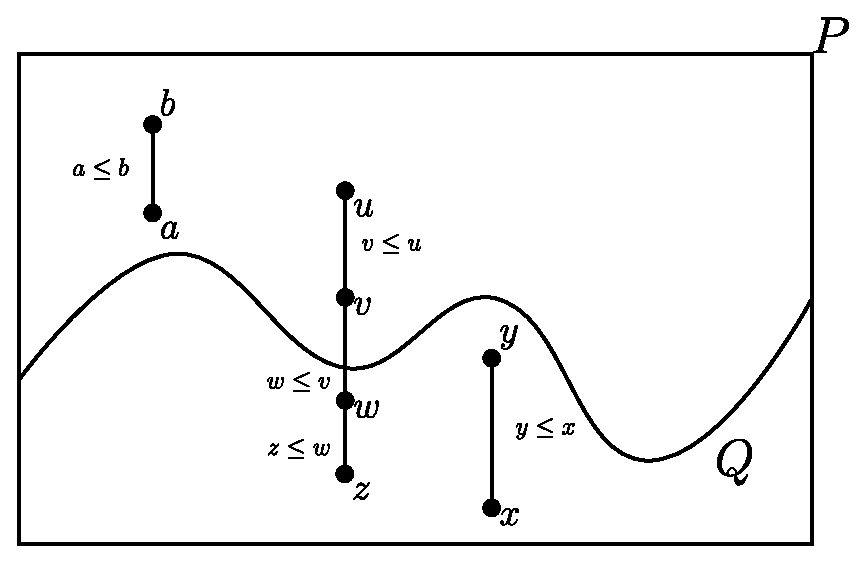
\includegraphics[scale=0.5]{./figures/Chapter1/up_down_sets.eps}
  \caption{$Q$ is a down-set of $P$ if, and only if $\com{P}{Q}$ is an
  up-st of $P$.}
  \label{figure_1.6}
\end{figure}

\begin{proposition}\label{proposition_1.6.5}
  Let $P$ be a poset. Then the following are true:
  \begin{enumerate}
    \item[(1)] $\Oc(P \oplus \mathbf{1}) \simeq \Oc(P) \oplus
      \mathbf{1}$. and $\Oc(\mathbf{1} \oplus P) \simeq \mathbf{1}
      \oplus \Oc(P)$.

    \item[(2)] If $P_1, P_2 \subseteq P$, then $\Oc(P_1 \cup P_2)
      \simeq \Oc(P_1) \times \Oc(P_2)$.
  \end{enumerate}
\end{proposition}
\begin{proof}
  Let $Q \in \Oc(P \oplus \mathbf{1})$, and take $x \in Q$ and $y \in
  P \oplus \mathbf{1}$ such that $y \leq x$. Then $y \in Q$, and
  either $y=0$ or $y \neq 0$. This puts $Q \in \Oc(P) \oplus
  \mathbf{1}$. Define then
  \begin{aligned}
    \phi:\Oc(P \oplus \mathbf{1}) & \xrightarrow{} \Oc(P) \oplus \mathbf{1}  \\
          Q & \xrightarrow{} Q
  \end{aligned}
  Then $\phi$ is the required order-isomorphism.

  Similarly, if $Q \in \Oc(\mathbf{1} \oplus P)$, then $Q \in
  \mathbf{1} \oplus \Oc(P)$; moreover notice that $\emptyset \in
  \Oc(\mathbf{1} \oplus P)$. Then take
  \begin{aligned}
    \phi:\Oc(\mathbf{1} \oplus P) & \xrightarrow{} \mathbf{1} \oplus \Oc(P)  \\
          Q & \xrightarrow{} Q
  \end{aligned}
  then $\phi$ is the required order-isomorphism.

  Finally, define the mape
  \begin{aligned}
    \phi:\Oc(P_1 \cup P_2) & \xrightarrow{} \Oc(P_1) \times \Oc(P_2) \\
          Q & \xrightarrow{} (Q \cap P_1, Q \cap P_2)  \\
  \end{aligned}
  Let $Q$ be a down-set of  $P_1 \cup P_2$, and $x \in Q \cap P_1$, and take
  $y \in P_1$ such that $y \leq x$. Since $x \in Q$ and $Q$ is a
  down-set, then  $y \in Q$ so that $y \in Q \cap P_1$. This makes $Q
  \cap P_1$ a down-set of $P_1$. Likewise, $Q \cap P_2$ is a down-set
  of $P_2$. Therefore $\phi$ is well-defined, and moreover it is onto.
  Now, suppose that $\phi(Q)=\phi(R)$. Then $Q \cap P_1=R \cap P_1$
  and $Q \cap P_2=R \cap P_2$, so that $Q=R$ and $\phi$ is 1--1. It
  remains that under the order of $\Oc(P_1) \times \Oc(P_2)$ that if
  $Q \subseteq R$ in $\Oc(P_1 \cup P_2)$, then $\phi(Q) \leq \phi(R)$.
  So $\phi$ is the required order-isomorphism.
\end{proof}

\begin{example}\label{example_1.14}
  \begin{enumerate}
    \item[(1)] Let $P_1$ and $P_2$ be according to the following
      diagram.
      \[\begin{tikzcd}[sep = scriptsize]
        &&&&&&&& \bullet \\
        & {P_1} &&&&&& \bullet & \bullet & \bullet \\
        & \bullet && \bullet && \bullet & \bullet & \bullet & \bullet & \bullet \\
        && \bullet && \bullet && \bullet & \bullet & \bullet && \bullet \\
        &&& \bullet && \bullet && \bullet && \bullet \\
        &&&&& \bullet &&& \bullet \\
        \bullet & \bullet & \bullet & \bullet & \bullet & \bullet &&& \bullet \\
        && \bullet & {P_2} & \bullet & \bullet & \bullet && {\Oc(P_1)}
        \arrow[no head, from=2-8, to=1-9]
        \arrow[no head, from=2-9, to=1-9]
        \arrow[no head, from=2-10, to=1-9]
        \arrow[no head, from=3-7, to=2-8]
        \arrow[no head, from=3-8, to=2-8]
        \arrow[no head, from=3-8, to=2-9]
        \arrow[no head, from=3-9, to=2-10]
        \arrow[no head, from=3-10, to=2-9]
        \arrow[no head, from=3-10, to=2-10]
        \arrow[no head, from=4-3, to=3-2]
        \arrow[no head, from=4-3, to=3-4]
        \arrow[no head, from=4-5, to=3-6]
        \arrow[no head, from=4-7, to=3-7]
        \arrow[no head, from=4-7, to=3-8]
        \arrow[no head, from=4-8, to=3-7]
        \arrow[no head, from=4-8, to=3-9]
        \arrow[no head, from=4-9, to=3-8]
        \arrow[no head, from=4-9, to=3-9]
        \arrow[no head, from=4-9, to=3-10]
        \arrow[no head, from=4-11, to=3-10]
        \arrow[no head, from=5-4, to=4-3]
        \arrow[no head, from=5-4, to=4-5]
        \arrow[no head, from=5-6, to=6-6]
        \arrow[no head, from=5-8, to=4-7]
        \arrow[no head, from=5-8, to=4-8]
        \arrow[no head, from=5-8, to=4-9]
        \arrow[no head, from=5-10, to=4-9]
        \arrow[no head, from=5-10, to=4-11]
        \arrow[no head, from=6-6, to=7-6]
        \arrow[no head, from=6-9, to=5-8]
        \arrow[no head, from=6-9, to=5-10]
        \arrow[no head, from=7-6, to=8-5]
        \arrow[no head, from=7-6, to=8-6]
        \arrow[no head, from=7-6, to=8-7]
        \arrow[no head, from=7-9, to=6-9]
        \arrow[no head, from=8-3, to=7-1]
        \arrow[no head, from=8-3, to=7-2]
        \arrow[no head, from=8-3, to=7-3]
        \arrow[no head, from=8-3, to=7-4]
        \arrow[no head, from=8-3, to=7-5]
      \end{tikzcd}\]
      Then $P_1 \simeq \mathbf{1} \oplus ((\mathbf{1} \oplus
      \bar{\mathbf{2}}) \uplus \mathbf{2})$, and $\Oc(P_1) \simeq
      \mathbf{1} \oplus ((\mathbf{1} \oplus \mathbf{2}^2) \times
      \mathbf{3})$.

    \item[(2)] Let $P_2$ be as in the above diagram. Then $\Oc(P_2)
      \simeq (\mathbf{1} \oplus \mathbf{2}^5) \times (\mathbf{2}^3
      \oplus \mathbf{3})$, and $|\Oc(P_2)|=(1+2^5) \cdot (2^3+3)=363$.
  \end{enumerate}
\end{example}
